%%*****************************************************************************
\SVN$Id: section-ide-jude.tex 7892 2009-08-07 14:37:56Z gene $
%%*****************************************************************************
%%
%% Copyright (C) 2005-2008 The ExTeX Group and individual authors listed below
%%
%% This library is free software; you can redistribute it and/or modify it
%% under the terms of the GNU Lesser General Public License as published by the
%% Free Software Foundation; either version 2.1 of the License, or (at your
%% option) any later version.
%%
%% This library is distributed in the hope that it will be useful, but WITHOUT
%% ANY WARRANTY; without even the implied warranty of MERCHANTABILITY or
%% FITNESS FOR A PARTICULAR PURPOSE. See the GNU Lesser General Public License
%% for more details.
%%
%% You should have received a copy of the GNU Lesser General Public License
%% along with this library; if not, write to the Free Software Foundation,
%% Inc., 59 Temple Place, Suite 330, Boston, MA 02111-1307 USA
%%
%%*****************************************************************************
%% @author Gerd Neugebauer
%%-----------------------------------------------------------------------------
\section{Modelling: Jude}

Jude is a UML modeller written in Java. It is distributed in a
community edition for free use. Currently the version 1.6.2 is
available from \url{http://www.esm.jp/jude-web/index.html}. 
\begin{figure}[thp]
  \centering
  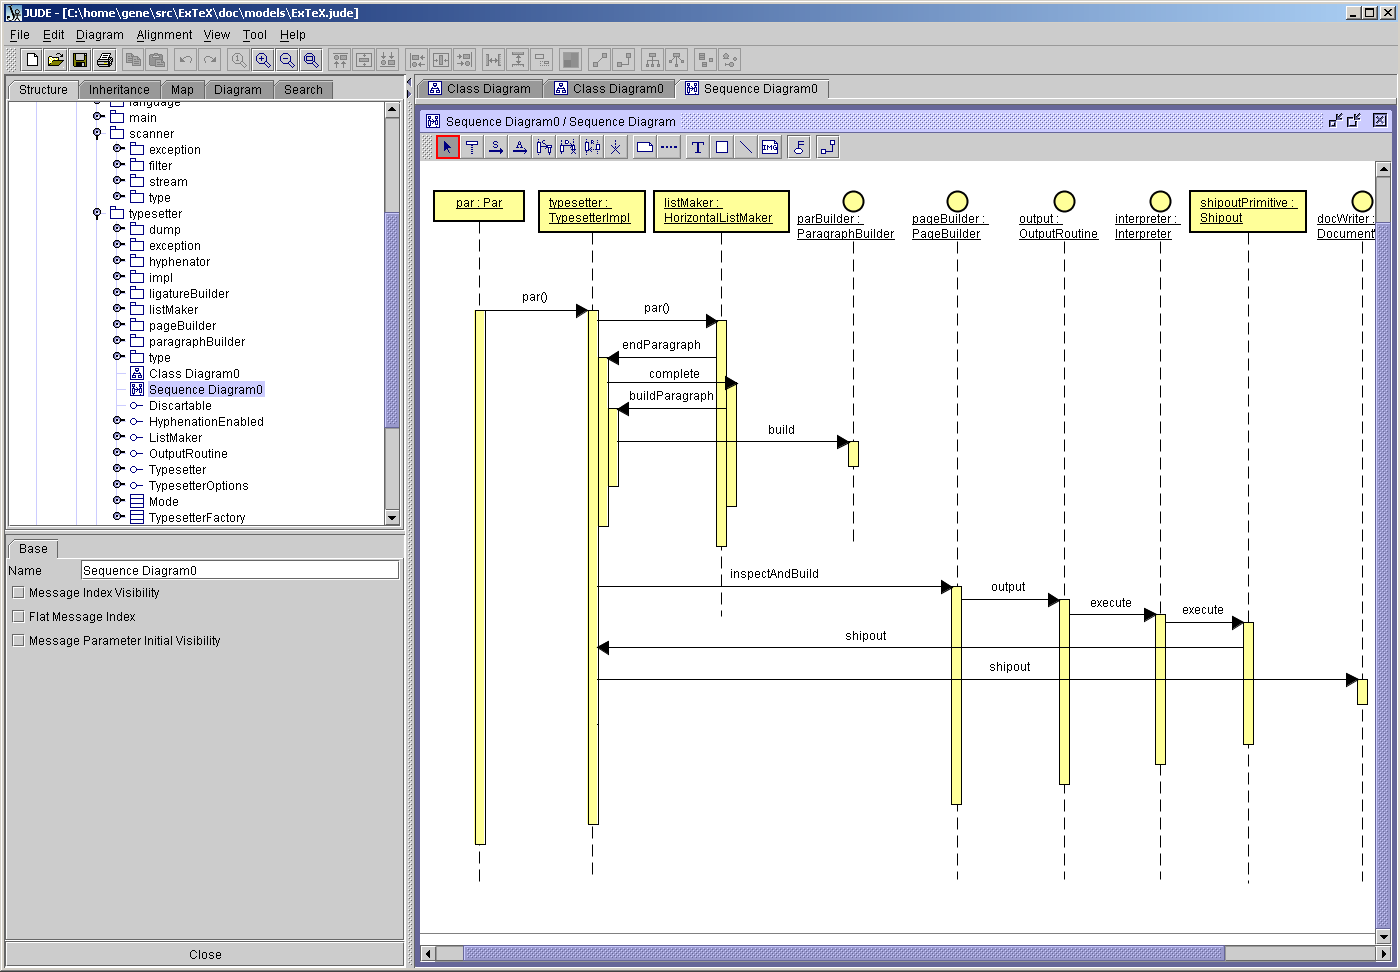
\includegraphics[width=\textwidth]{image/jude-seq}
  \caption{Jude}\label{fig:jude}
\end{figure}

Jude should be used for any situations where UML diagrams are needed.
A screenshot of Jude can be seen in figure~\ref{fig:jude}.

Models for \ExTeX\ should be placed in the directory \File{doc/models}.

